\documentclass[11pt]{article}

\usepackage[utf8]{inputenc}
\usepackage[spanish]{babel}
\decimalpoint

\usepackage{csquotes}
\usepackage[T1]{fontenc}
\usepackage{lmodern}
\usepackage[a4paper, total={6.7in, 11in}]{geometry}
\usepackage{amsmath}
\usepackage{amssymb}
\usepackage[per-mode=fraction, inter-unit-product=\cdot, quotient-mode=fraction]{siunitx}
\usepackage{float}
\usepackage{hyperref}
\usepackage{xcolor}
\usepackage{tablefootnote}
\usepackage{chemformula}

\usepackage[shortlabels]{enumitem}
\setlist{listparindent=\parindent}

\newcommand*\diff{\mathop{}\!\mathrm{d}}
\newcommand{\inv}[1]{\frac{1}{#1}}
\newcommand{\deriv}[2]{\dfrac{\diff #1}{\diff #2}}
\newcommand{\ROM}[1]{%
  \textup{\uppercase\expandafter{\romannumeral#1}}%
}

\usepackage{graphicx}
\graphicspath{{./}}

\begin{document}

	\begin{table}
		\centering
		\begin{tabular}{|p{4.2cm}|l|l|}
			\hline
			Propiedad & NPN & PNP \\
			\hline
			&&\\
			\textbf{Región activa directa}
			& $V_{BE} > 0 \land V_{BC} < 0$
			& $V_{EB} > 0 \land V_{CB} < 0$ \\
			& $I_C = I_S\left(e^{\frac{V_{BE}}{V_t}} - 1\right)$\color{red}{$\left(1 + \dfrac{V_{CE}}{V_A}\right)$}
			& $I_C = I_S\left(e^{\frac{V_{EB}}{V_t}} - 1\right)$\color{red}{$\left(1 + \dfrac{V_{EC}}{V_A}\right)$} \\
			&&\\
			\hline
			&&\\
			\textbf{Corriente de diodo en directa Ebers--Moll}
			& $I_F = I_{ES}\left(e^{\frac{V_{BE}}{V_t}} - 1\right)$
			& $I_F = I_{ES}\left(e^{\frac{V_{EB}}{V_t}} - 1\right)$ \\
			&&\\
			\hline
			&&\\
			\textbf{Corriente de diodo en reversa Ebers--Moll}
			& $I_R = I_{CS}\left(e^{\frac{V_{BC}}{V_t}} - 1\right)$
			& $I_R = I_{CS}\left(e^{\frac{V_{CB}}{V_t}} - 1\right)$ \\
			&&\\
			\hline
			&&\\
			\textbf{Corriente de colector Ebers--Moll}
			& $I_C = \alpha_F I_F - I_R$
			& $I_C = I_R - \alpha_F I_F$ \\
			&&\\
			\hline
			&&\\
			\textbf{Corriente de emisor Ebers--Moll}
			& $I_E = \alpha_R I_R - I_F$
			& $I_E = I_F - \alpha_R I_R$ \\
			&&\\
			\hline
			&\multicolumn{2}{|c|}{} \\
			\textbf{Relación de reciprocidad}
			& \multicolumn{2}{|c|}{$\alpha_F I_{ES} = \alpha_R I_{CS}$} \\
			&\multicolumn{2}{|c|}{} \\
			\hline
		\end{tabular}
		\caption{Transistores BJT}
	\end{table}

	\begin{table}
		\centering
		\begin{tabular}{|p{7cm}|l|}
			\hline
			Parámetro & Expresión \\
			\hline
			&\\
			\textbf{LCK en BJT} & $I_E = I_C + I_B$ \\
			&\\
			\hline
			&\\
			\textbf{Corriente de fuga en reversa}\tablefootnote{$A_E$ se suma al
			colocar dos transistores BJT en paralelo.}
			[\si{\ampere}] & $I_S = \dfrac{A_E q D_n n_i^2}{N_B W_B}$ \\
			&\\
			\hline
			&\\
			\textbf{Ganancia de corriente de emisor común} [adimensional] & $\beta = \dfrac{I_C}{I_B}$ \\
			& $\beta = \dfrac{\alpha}{1 - \alpha}$ \\
			&\\
			\hline
			&\\
			\textbf{Ganancia de corriente de base común} [adimensional] & $\alpha = \dfrac{I_C}{I_E}$ \\
			& $\alpha = \dfrac{\beta}{\beta + 1}$ \\
			&\\
			\hline
			&\\
			\textbf{Transconductancia} [\si{\siemens}] & $g_m = \dfrac{I_C}{V_t}$ \\
			&\\
			\hline
			&\\
			\textbf{Resistencia de base} [\si{\ohm}] & $r_\pi = \dfrac{\beta}{g_m}$ \\
			&\\
			\hline
			&\\
			\textbf{Resistencia de salida} [\si{\ohm}] & $r_o = \dfrac{V_A}{I_C}$ \\
			&\\
			\hline
			&\\
			\textbf{Condición de saturación débil} & $V_{BE} > 0 \land V_C > V_B - \SI{200}{mV}$ \\
			&\\
			\hline
			&\\
			\textbf{Condición de activa directa Ebers--Moll} & $I_R = 0$ \\
			&\\
			\hline
			&\\
			\textbf{Condición de activa reversa Ebers--Moll} & $I_F = 0$ \\
			&\\
			\hline
		\end{tabular}
		\caption{Parámetros BJT}
	\end{table}

	\begin{table}
		\centering
		\begin{tabular}{|l|l|}
			\hline
			&\\
			\textbf{Permitividad del vacío} & $\varepsilon_0 = \SI{8.854e-14}{\farad\per\centi\meter}$ \\
			&\\
			\hline
			&\\
			\textbf{Permitividad relativa del \ch{SiO2}} & $\varepsilon_{ox} = \num{3.9}$ \\
			&\\
			\hline
			&\\
			\textbf{Voltaje térmice} & $V_t = \dfrac{kT}{q} = \SI{26}{mV}$ (a \SI{300}{K}) \\
			&\\
			\hline
		\end{tabular}
		\caption{Constantes}
	\end{table}

	\begin{table}[h]
		\centering
		\begin{tabular}{|l|c|c|c|}
			\hline
			Región de operación & $C_{GD}$ & $C_{GB}$ & $C_{GS}$ \\
			\hline
			&&&\\
			Subumbral & $C_{OV}$ & $C_{OX}$ & $C_{OV}$ \\
			&&&\\
			\hline
			&&&\\
			Triodo & $\frac{1}{2}C_{OX}$ & $C_{OX}$ & $\frac{1}{2}C_{OX}$ \\
			&&&\\
			\hline
			&&&\\
			Saturación & $C_{OV}$ & $C_{OX}$ & $\frac{2}{3}C_{OX}$ \\
			&&&\\
			\hline
		\end{tabular}
		\caption{Capacitancias parásitas \tablefootnote{Todas las capacitancias
		que no se enuncien aquí se asumen nulas.}}
	\end{table}

	\begin{table}
		\centering
		\begin{tabular}{|p{3cm}|c|c|c|}
			\hline
			Propiedad & Common emitter & Common base & Eitter follower \\
			\hline
			&&&\\
			\textbf{Caso estudiado}
			& 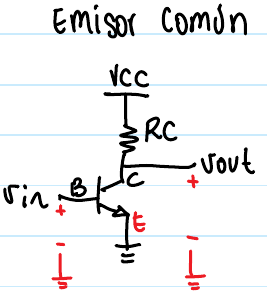
\includegraphics[width=0.20\textwidth, keepaspectratio]{ce}
			& 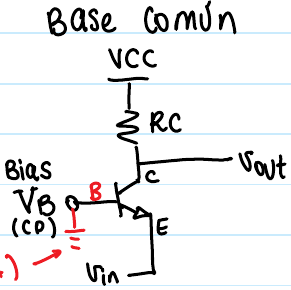
\includegraphics[width=0.20\textwidth, keepaspectratio]{cb}
			& 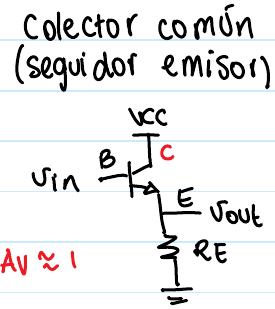
\includegraphics[width=0.20\textwidth, keepaspectratio]{cc} \\
			&&&\\
			\hline
			&&&\\
			\textbf{Ganancia} [\si{\volt/\volt}] & $A_v = -g_m R_C$ & $A_v = g_m R_C$ & $A_v = \dfrac{R_E}{\frac{1}{g_m} + R_E} \approx 1$ \\
			&&&\\
			\hline
			&&&\\
			\textbf{Impedancia de entrada} [\si{\ohm}] & $R_{in} = r_\pi$ & $R_{in} = \frac{1}{g_m}\parallel r_\pi$\tablefootnote{Si $\frac{1}{g_m} \ll r_\pi$, se puede aproximar como $r_{\text{in}} = \frac{1}{g_m}$.} & $R_{in} = r_\pi + R_E(\beta + 1)$ \\
			&&&\\
			\hline
			&&&\\
			\textbf{Impedancia de salida} [\si{\ohm}] & $R_{out} = R_C$ & $R_{out} = R_C$ & $R_{out} = R_E\parallel\frac{1}{g_m}$ \\
			&&&\\
			\hline
		\end{tabular}
		\caption{Topologías de amplificadores BJT}
	\end{table}

	\begin{table}
		\centering
		\begin{tabular}{|p{0.3\textwidth}|p{0.3\textwidth}|}
			\hline
			&\\
			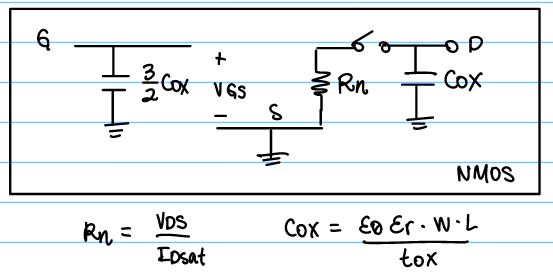
\includegraphics[width=0.3\textwidth, keepaspectratio]{digital-model}
			& 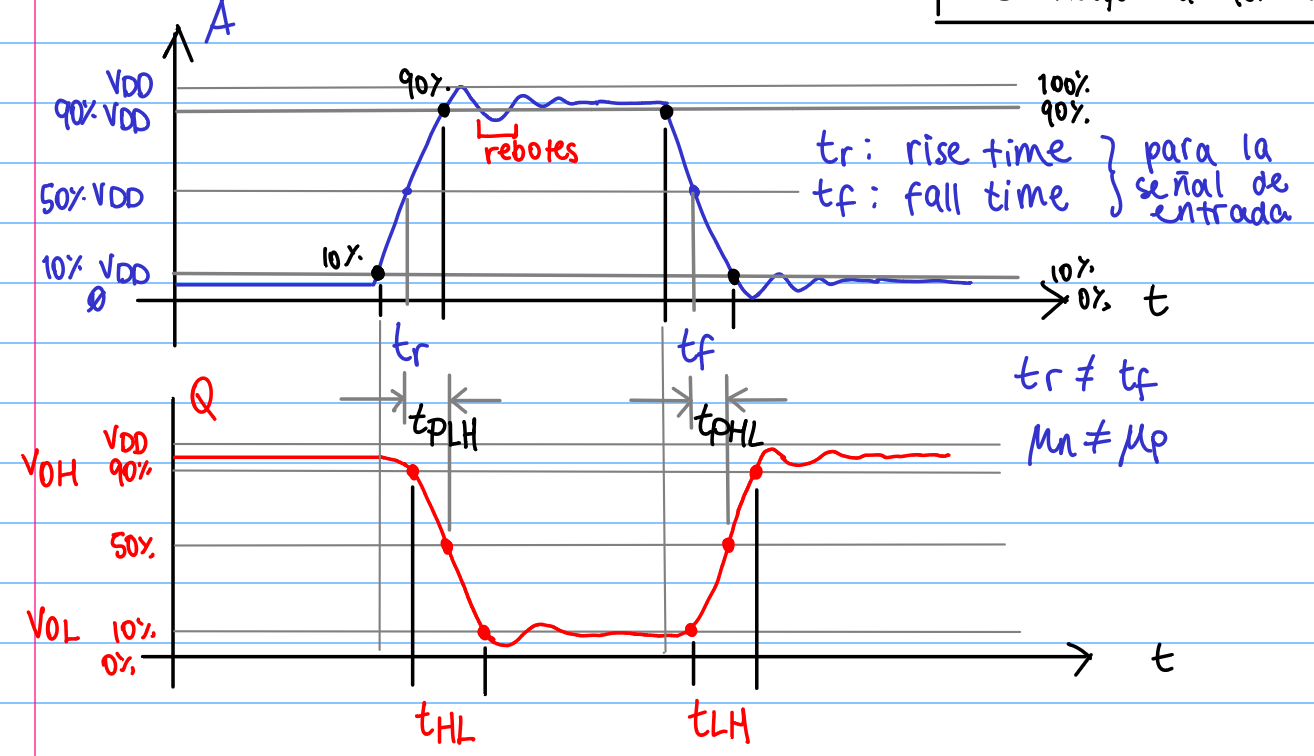
\includegraphics[width=0.3\textwidth, keepaspectratio]{digital-timings} \\
			\textbf{Modelo digital del MOSFET}
			& \textbf{Tiempos de respuesta}\tablefootnote{La señal se considera $0$ lógico
			si su amplitud es menor que \SI{10}{\percent} de $V_{DD}$ y $1$ lógico
			si es mayor que el \SI{90}{\percent}.} \\
			&\\
			\hline
		\end{tabular}
		\caption{Lógica digital}
	\end{table}

	\begin{table}
		\centering
		\begin{tabular}{|p{0.25\textwidth}|p{0.25\textwidth}|p{0.25\textwidth}|}
			\hline
			&\\
			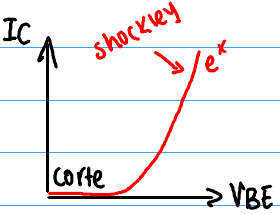
\includegraphics[width=0.25\textwidth, keepaspectratio]{transfer}
			& 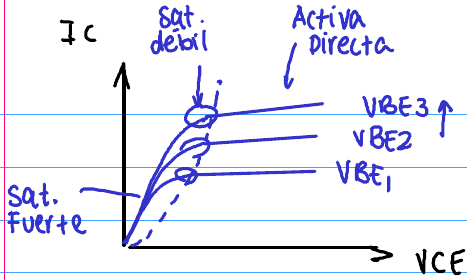
\includegraphics[width=0.25\textwidth, keepaspectratio]{output}
			& 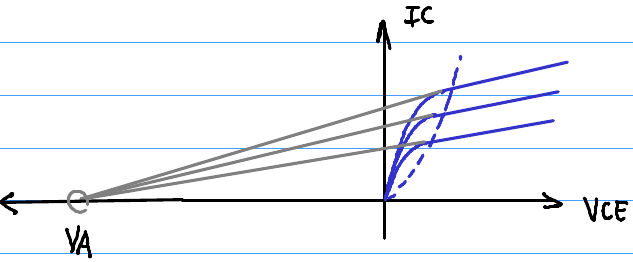
\includegraphics[width=0.25\textwidth, keepaspectratio]{early} \\
			\textbf{Curva de transferencia} & \textbf{Curva de salida} & \textbf{Efecto Early} \\
			&\\
			\hline
			&\\
			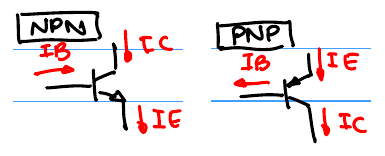
\includegraphics[width=0.25\textwidth, keepaspectratio]{simbologia}
			& 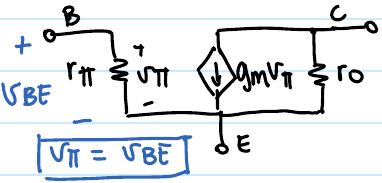
\includegraphics[width=0.25\textwidth, keepaspectratio]{smallsignal-npn}
			& 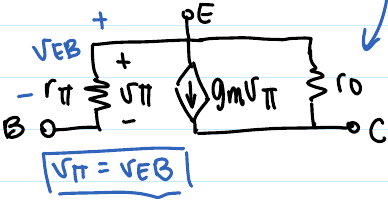
\includegraphics[width=0.25\textwidth, keepaspectratio]{smallsignal-pnp} \\
			\textbf{Simbología} & \textbf{Modelo de pequeña señal NPN} & \textbf{Modelo de pequeña señal PNP} \\
			&\\
			\hline
			&\\
			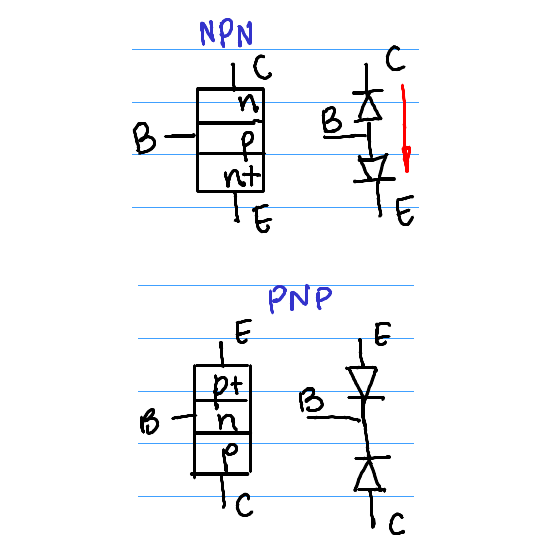
\includegraphics[width=0.25\textwidth, keepaspectratio]{diodes}
			& 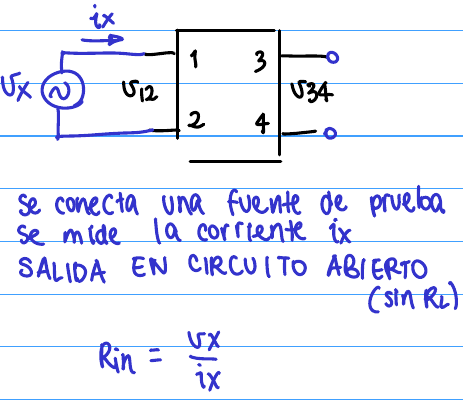
\includegraphics[width=0.25\textwidth, keepaspectratio]{input-impedance}
			& 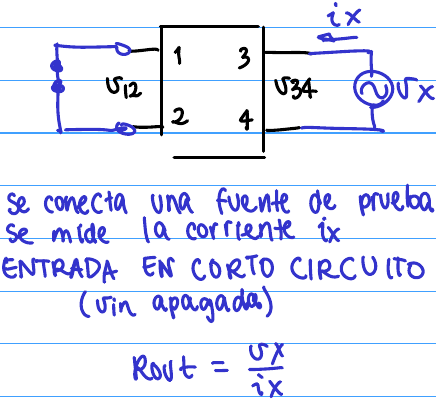
\includegraphics[width=0.25\textwidth, keepaspectratio]{output-impedance} \\
			\textbf{Modelo de diodos} & \textbf{Impedancia de entrada} & \textbf{Impedancia de salida} \\
			&\\
			\hline
		\end{tabular}
		\caption{Gráficas y modelos BJT}
	\end{table}

	\begin{table}
		\centering
		\begin{tabular}{|c|c|}
			\hline
			&\\
			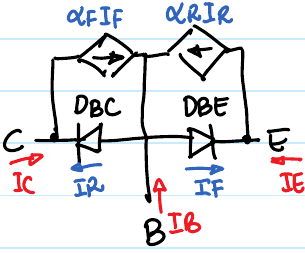
\includegraphics[width=0.3\textwidth, keepaspectratio]{em-npn}
			& 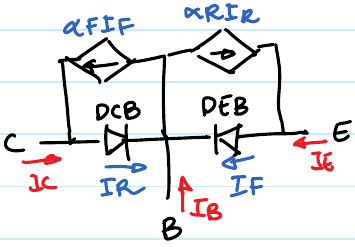
\includegraphics[width=0.3\textwidth, keepaspectratio]{em-pnp} \\
			Modelo completo NPN & Modelo completo PNP \\
			&\\
			\hline
			&\\
			{\begin{minipage}{0.5\textwidth}$$\begin{cases}
				I_C &= \alpha_F I_{ES}\left(e^{\frac{V_{BE}}{V_t}} - 1\right) - I_{CS}\left(e^{\frac{V_{BC}}{V_t}} - 1\right) \\
				I_E &= \alpha_R I_{CS}\left(e^{\frac{V_{BC}}{V_t}} - 1\right) - I_{ES}\left(e^{\frac{V_{BE}}{V_t}} - 1\right) \\
			\end{cases}$$\end{minipage}}
			& {\begin{minipage}{0.5\textwidth}$$\begin{cases}
				I_C &= I_{CS}\left(e^{\frac{V_{CB}}{V_t}} - 1\right) - \alpha_F I_{ES}\left(e^{\frac{V_{V_{EB}}}{V_t}} - 1\right) \\
				I_E &= I_{ES}\left(e^{\frac{V_{EB}}{V_t}} - 1\right) - \alpha_R I_{CS}\left(e^{\frac{V_{V_{CB}}}{V_t}} - 1\right)
			\end{cases}$$\end{minipage}} \\
			&\\
			\hline
		\end{tabular}
		\caption{Modelos de Ebers--Moll \tablefootnote{Solo es necesario en las
		regiones que \textbf{no} son activa directa ni saturación débil, pero sí
		en activa reversa y saturación fuerte. Puede usarse en cualquier región.}}
	\end{table}

\end{document}
